\documentclass[preprint]{elsarticle}
\biboptions{round, numbers}
\usepackage[latin1]{inputenc}
%\usepackage[T1]{fontenc}
%\usepackage{textcomp}
\usepackage{graphicx}
\usepackage{color}
%\usepackage{setspace}
\usepackage{url}
\usepackage[english]{babel}


\begin{document}

%%%%%%%%%%%%%%%%%%%%%%%%%%%%%%%   TITLE   %%%%%%%%%%%%%%%%%%%%%%%%%%%%%%%

\title{A review on BYOD solutions and corporate security systems}

%%%%%%%%%%%%%%%%%%%%%%%%%%%%%%%   AUTHORS   %%%%%%%%%%%%%%%%%%%%%%%%%%%%%%%

\author{P. de las Cuevas}
\ead{paloma@geneura.ugr.es}
\address{Departamento de Arquitectura y Tecnolog�a de Computadores. Escuela T�cnica Superior de Ingenier�as Inform�tica y de Telecomunicaci�n. CITIC. University of Granada, Spain}
\author{A. M. Mora}
\ead{amorag@geneura.ugr.es}
\address{Departamento de Arquitectura y Tecnolog�a de Computadores. Escuela T�cnica Superior de Ingenier�as Inform�tica y de Telecomunicaci�n. CITIC. University of Granada, Spain}

\maketitle

%
%%%%%%%%%%%%%%%%%%%%%%%%%%%%%%%%%   ABSTRACT   %%%%%%%%%%%%%%%%%%%%%%%%%%%%%%%%%
%
\begin{abstract} 
Enterprises, and their Chief Security Officers (CSOs) particularly, want to be sure that their security policies are complied. This goal turned hard to achieve since employees are able to use their own devices (laptops, smartphones, and tablets) at work, or at home but for work purposes. As this is part of the Bring Your Own Device (BYOD) philosophy and is being adopted by many companies everyday, a number of solutions have arisen in order to adapt it securely. In this paper, the most relevant solutions are presented, and so is displayed the European MUSES (Multiplatform Usable Endpoint Security) project, which tries to go further taking into account user behaviour for security rules adaption.
\end{abstract}

%
%%%%%%%%%%%%%%%%%%%%%%%%%%%%%%%%%   KEYWORDS   %%%%%%%%%%%%%%%%%%%%%%%%%%%%%%%%%
%
\begin{keyword}
BYOD \sep Corporate mobile security \sep End-to-end security solutions
\end{keyword}

%
%%%%%%%%%%%%%%%%%%%%%%%%%%%%%%%   INTRODUCTION   %%%%%%%%%%%%%%%%%%%%%%%%%%%%%%%
%
\section{Introduction}
\label{sec:intro}

The rest of the paper is organized as follows. First, some background situation about corporate secure networks is presented in section \ref{sec:preliminaryconcepts}, explaining how BYOD affects to them. Then, some solutions from different companies are detailed in section \ref{sec:toolsreview}, being specified for each one if the correspondent tool is available or, if not, the aproximate release date. Some solutions are focused only in smartphones, while others are thought for laptops; also some are for a certain platform, but others remain multiplatform. Finally, the conclusions are discussed in section \ref{sec:conclusions}.

%
%%%%%%%%%%%%%%%%%%%%%%%%%%%%%%%   BACKGROUND  %%%%%%%%%%%%%%%%%%%%%%%%%%%%%%%
%
\section{Preliminary concepts and background about enterprise security}
\label{sec:preliminaryconcepts}

Until these days, enterprises used to follow a static policy devoted to controlling a certain structure, where the assets and the devices were purchased and maintained by the company. Now that corporate networks are becoming dynamic for being adapted to the BYOD philosophy, there is an additional risk because the devices that the employees use are not always company-owned.

On the other hand, employee-owned devices like smartphones, they are not just for work purposes anymore. As the name says, smartphones are more than simple old cell phones, and people who use them in their works have the possibility of having a good balance between work and private life. For this reason, the risk of uncontrolled devices accessing to corporate access in unsafe conditions, due to the number of risky applications, is bigger.

Then, it is necessary to take into account the security in an outsourced enterprise model. Figure \ref{fig:outsourced_sol_img} presents an example situation in which some of the mobile services have been outsourced to an external operator, typically a telecommunications operator.
The functional elements are the same ones as in an enterprise managed solution. For instance, the demilitarized zone, the intranet wired and WiFi zones, the Intrusion Detection System (IDS), or the mail and VPN servers. However some of them have been moved outside the enterprise. Of course the moved elements try to exemplify the most typical outsourced components for enterprises having a mobile device strategy.
The main differences are related to the possible outsourcing of the:

\begin{enumerate}
	\item \textbf{Network Access Control (NAC):} it checks that mobile devices satisfy a set of prerequisites (e.g., OS patch level, antivirus properties, etc.) before allowing them connecting to the intranet. Normally it manages the accesses to the Intranet WiFi net, but it can also be involved in controlling Virtual Private Network (VPN) accesses.
	\item \textbf{Active Directory Domain Controller (ADDC):} this service exemplifies the network management framework in charge of authenticating devices and users, as well as of distributing enterprise security policies.
	\item \textbf{MDM Server:} many telecommunications operators are deploying Machine-to-Machine (M2M) management frameworks, and start offering related services that, among other features, provide features for managing mobile devices. The telecommunications operators can play a relevant role especially in BYOD scenarios due to their habits of subscription plans including medium-to-high end smart phones or tablets;
	\item \textbf{Applications Store:} there is a big interest of telecommunications operators for the so called mobile ecosystem, i.e. services tied to mobile devices and to mobile device apps. One of the key elements of this mobile ecosystem is the controlled provisioning of apps or content targeted to meet enterprise requirements, especially Small and Medium Enterprises (SME). In figure \ref{fig:outsourced_sol_img} the telecommunications operator manages a Private/Hybrid App Store to exemplify both situations in which the operated App Store provides and manages exclusively enterprise specific apps (Private Application Store), as well as enterprise and operator or third parties apps (Hybrid App Store).
	\item \textbf{Mail Server:} enterprises having a consistent base of employees or collaborators using mobile devices often prefer the outsourcing of the enterprise mail service (or use fully outsourced Productivity Suites) to reduce costs, configuration and management issues, and improve service quality.
\end{enumerate}

\begin{figure}
	\begin{center}
		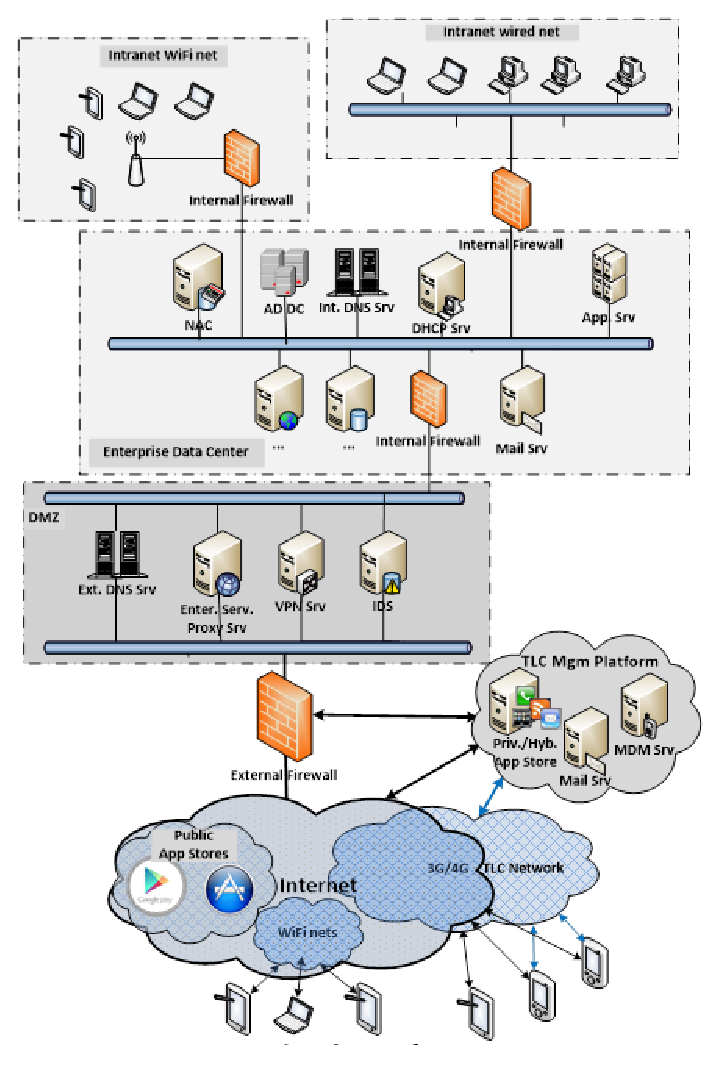
\includegraphics[scale=0.6]{img/outsourced_solution.eps}
		\caption{Security architecture model of an enterprise in which some of the mobile services have been outsourced to an external operator.}
	\label{fig:outsourced_sol_img}
	\end{center}
\end{figure}

%
%%%%%%%%%%%%%%%%%%%%%%%%%%%%%%%   TOOLS REVIEW  %%%%%%%%%%%%%%%%%%%%%%%%%%%%%%%
%

\section{Tools for corporate mobile security}
\label{sec:toolsreview}

Now that BYOD philosophy is a trend, a number of tools have been designed specifically for CSOs and Chief Information Security Officers (CISOs) to secure, monitor, and control spartphones and other personal mobile or portable devices. Some of these tools have influenced the development of the European MUSES project itself, showed in \ref{subsec:muses}. This section presents the products that can be considered related to MUSES objectives.

% Don't completely like the intro for being too focused to MUSES.

%----------------------------------------------------------------------------
\subsection{IBM Hosted Mobile Device Security Management}
\label{subsec:ibm}

One of the first companies who supported the BYOD model was IBM in 2011, as they recognized the increase of employees who brang their personal smartphones or tablets into the workplace. To help organizations embrace both company and employee owned mobile devices (as said, this practise is part of the BYOD model) in a security-rich environment, IBM developed a mobile device security management solution. For IBM, a mobile security strategy should focus on several key areas.

On one hand, the organization should identify which business data the strategy will allow to be stored and processed on which mobile devices. This helps determine what needs to be protected and to what degree. Then, because different mobile platforms have different native security mechanisms, the organization needs to define which mobile device platforms will be allowed in the business environment and, thus, need to be supported in the mobile security strategy and plan. Also there is need to decide the responsibility for mobile security management work, whether using the current IT security team to handle mobile devices, or outsourcing to a managed security service provider. And no matter what the mobile environment, a number of mobile security policies and best-practise procedures need to be put in place and should also be identified in the company's mobile security strategic plan.

Taking into account these considerations, IBM developed a framework that specifies security domains and levels for applying various security technologies. When applied to mobile devices, the framework suggests the following security controls, with actual requirements varying by deployment. The features of this framework are detailed in table \ref{tab:IBMframework}.

%HACER UNA TABLA
%No s� c�mo bajar la tabla �eeee~

\begin{table}
	\caption{IBM Hosted Mobile Device Security Management framework}
	\label{tab:IBMframework}
	\begin{tabular}{| p{11cm} |}
		\hline
		\textbf{Identity and access}\\
		\hline
		Enforce strong passwords to access the device.\\
		\hline
		Use site authentication or two-factor user authentication to help increase the trustworthiness between a user and a website.\\
		\hline
		If VPN access to corporate intranet is allowed, include capability to control what IP addresses can be accessed and when re-authentication is required for accessing critical resources.\\
		\hline
		\hline
		\textbf{Data protection}\\
		\hline
		Encrypt business data stored on the device and during transmission.\\
		\hline
		Include capability to wipe data locally and remotely.\\
		\hline
		Set timeout to lock the device when it is not used.\\
		\hline
		Periodically back up data on the device so data restore is possible after the lost device has been recovered.\\
		\hline
		Include capability to locate or lockout the device remotely.\\
		\hline
		\hline
		\textbf{Application security}\\
		\hline
		Download business applications from controlled locations.\\
		\hline
		Run certified business applications only.\\
		\hline
		Monitor installed applications and remove those identified to be untrustworthy or malicious.\\
		\hline
		\hline
		\textbf{Fundamental integrity control}\\
		\hline
		Run antimalware software to detect malware on storage and in memory.\\
		\hline
		Run a personal firewall to filter inbound and outbound traffic.\\
		\hline
		Integrate with the company's VPN gateway so a device's security posture becomes a dependency for intranet access.\\
		\hline
		\hline
		\textbf{Governance and compliance}\\
		\hline
		Incorporate mobile security into the company's overall risk management program.\\
		\hline
		Run a personal firewall to filter inbound and outbound traffic.\\
		\hline
		Include mobile devices in the company's periodic security audit.\\
		\hline
	\end{tabular}
\end{table}

Regarding IBM hosted mobile device security solution's architecture, the solution is built on a sound client-server architecture in which the server centrally controls and manages security policies and settings for various security features. The client would be installed on the mobile device and regularly communicate with the server to enforce policies, execute commands and report status. Also, IBM's solution contains reporting and analysis capabilities, with information that helps the company to support policy and regulation compliance, recognize the mobile threat landscape and evaluate the solution's effectiveness in countering threats.

%----------------------------------------------------------------------------
\subsection{Sophos Mobile Control}
\label{subsec:sophos}

Sophos is a company founded in 1985 focused on IT security and data protection for businesses. Their \"Mobile Device Management\" main product is Sophos Mobile Control.
Sophos Mobile Control is oriented to IT administration for mobile devices. Sophos offers to the users the possibility of choosing the delivery model to suit their needs, i.e., between on-premise and Software as a Service (SaaS). The features of this tool are the following:

\begin{enumerate}
	\item Mobile Device Management � The tool offers the possibility of managing all workers and co-workers smartphones and tablets from a single-based console. The console monitors the devices throughout their full lifecycle: from the initial set up and enrolment, right through to decommissioning. Other features are:
	
	\begin{enumerate}
		\item It is possible also to connect to an existing user directory using Lightweight Directory Access Control (LDAP). LDAP is an application protocol for accessing and maintaining distributed directory information services over an Internet Protocol (IP) network.
		\item Configure policies for the devices and deploy them over the air.
		\item Turn on the built-in security features for iOS, Android, Windows and BlackBerry devices, including password protection and encryption.
		\item Drill down to the individual settings for all registered devices for configuration, serial numbers, model and hardware details, installed applications and much more.
		\item Manage your apps with an included Enterprise App Store.
		\item Use a dashboard to get the status of the devices at-a-glance.
		\item Define which features are available to the workers using a self-service portal.
		\item Initiate mitigation actions in case of loss or theft, such as lock, wipe, remote alarm and SIM change notification.
		\item Locate Android and iOS devices.
	\end{enumerate}
	
	\item Mobile Security � Additional security is provided by the incorporation of Malware and Web protection. Although, this feature is optional.
	\item Compliance Enforcement � The main goal is not to sacrifice company's security in favour of flexibility for the users. Company's BYOD initiative should include an Acceptable Use Policy to ensure the users are aware of any measures the company may take if a device breaches the security policies. This is reachable by doing three main tasks:	

	\begin{enumerate}
		\item Enforce Security Policies: Sophos Mobile Control allows setting up user and group-based security policies. The security settings can also vary from one platform to another. Set task bundles and individual actions for many different violations.
		\item Risk mitigation: these actions can be set according to the severity of a breach. For minor cases, the company may want to simply inform the user. If sensitive data is at risk, a remote wipe may be the only viable option. The actions vary for each platform, but the most common platforms such as Android and iOS allow blocking email access, notifying the admin, performing a remote lock or wiping, locating a device using 3D maps, triggering a remote alarm, transferring a task bundle combining a number of actions, and Sophos Mobile Security adds the possibility of trigger a scan.
		\item Compliance check: the settings available in the compliance check vary for each platform. Some of the most widely used features include allow or disallow root rights or jailbreaking, allow/disallow app downloads from non-market app stores, require encryption, and whitelist or blacklist apps. Additionally, Sophos Mobile Security allows disallowing malware apps, set maximum intervals since last Mobile Security scan, and allow or disallow suspicious apps and potentially unwanted apps (named PUAs).
	\end{enumerate}
	
	\item Mobile Application Management � The Enterprise App Store in Sophos Mobile Control allows the company to supply the users with recommended and required apps directly on their device. Both company's in-house and app store apps are shown on the user's mobile device, where they can click to trigger the installation.
	\item User Self-Service � One of company's goals is to keep the employees working without increasing the burden for the IT department. The self-service portal built-in included in Sophos Mobile Control has the following features:
	
	\begin{enumerate}
		\item Allow users to register their own devices and agree to an acceptable use policy that the company has defined.
		\item Let them use their personal device as part of the BYOD program, and the company can make sure it is secured.
		\item The users can choose to remotely locate, lock or wipe their devices and reset their passcode without having to contact the company help desk.
		\item Provide a simple step-by-step process when they register a device. All profiles, including email access, are available immediately after registration.
		\item The company define which features are available in its self-service portal from the administrator console.
		\item The users can access the portal from their mobile device or from any PC with Internet access.
	\end{enumerate}
	
	\item Easy configuration and maintenance � Sophos provides an easily install and maintain control with over-the-air setup and configuration from a web console.
	
\end{enumerate}

%----------------------------------------------------------------------------
\subsection{Good's Bring Your Own Device solution}
\label{subsec:goodsbyod}

Good Technology is a company that was founded in 1996 in California. They provide Push e-mail (for further explanation, see Chapter 8: Glossary), see and mobile device management and security products for mobile phones. The philosophy followed by Good is similar to Samsung's Knox one: to create a secure container that places an unreachable partition between personal and business data to protect email and other programs. The solutions that they offer are:

\begin{enumerate}
	\item Let the employees choose the smartphone, tablet, or other mobile device they want to use.
	\item Protect user privacy and critical information by using a secure container to separate personal and company data.
	\item Cut device and carrier costs by running a BYOD program that reduces the need for company-owned devices.
	\item Block unauthorized devices from the company's network by leveraging Good's secure Network Operations Center (NOC).
	\item Provide access to secure collaboration solutions (email, PIM, calendar), intranet, and in-house or third-party mobile applications.
	\item Offer best practice recommendations to help the company's bring-your-own-device policies such as reimbursements and stipends. There is a document available at Good's webpage (at \url{http://www1.good.com/mobility-management-solutions/bring-your-own-device}) which contains a number of questions about security policies and how to cope them all.
\end{enumerate}

%----------------------------------------------------------------------------
\subsection{Samsung's Knox Mobile Security Suite}
\label{subsec:samsungknox}

As part of its SAFE (Samsung for enterprise) brand, Samsung revealed at the Barcelona Mobile World Congress 2013 the Knox application, which will be available on his next Galaxy smartphone generation.
The main feature of this security package is the use of different containers for the business and the personal side. Each one even has its own set of wallpapers, in order to be more evident for the user. Figure \ref{fig:img_knox_01} shows the architecture followed by the application.
To enter the business side, it will be necessary to introduce a password. Nevertheless, no passwords will be required for the business applications anymore. The applications approved by the company IT department must meet Samsung's security standards and allow single sign-on. There will be over 338 IT policies that can be access via the Knox API. Also, Knox allows different VPNs for individual apps.
Regarding the information protection methods, data files saved by applications of each environment are encrypted with AES 256-bit algorithm, in such manner the container and only the container can access these files. In the same way, the user won't be able to share data between the two environments:

\begin{enumerate}
	\item There will be separate contact lists and the user cannot send a contact from one side to the other.
	\item If the user copies data to the clipboard in the Knox container, it won't be there in the personal container.
\end{enumerate}
 
Other features of this tool are the following:

\begin{enumerate}
	\item Customizable Secure Boot � This ensures that only verified and authorized software can run on the device. It is a primary component that forms the first line of defence against malicious attacks on devices with Samsung KNOX. In addition, Samsung Knox's Secure Boot technology allows the switch of the secure boot root certificate in a secure manner after the devices are shipped.
	\item TrustZone-based Integrity Measurement Architecture (TIMA) � This runs in the secure-world and provides continuous integrity monitoring of the Linux kernel. When TIMA detects that the integrity of the kernel or the boot loader is violated, it takes a policy-driven action in response. One of these policy actions disables the kernel and powers down the device.
	\item Security Enhancements for Android � This feature provides an enhanced mechanism to enforce the separation of information based on confidentiality and integrity requirements. It isolates applications and data into different domains so that threats of tampering and bypassing of application security mechanisms are reduced while the amount of damage that can be caused by malicious or flawed applications is minimized.
\end{enumerate}

\begin{figure}
	\begin{center}
		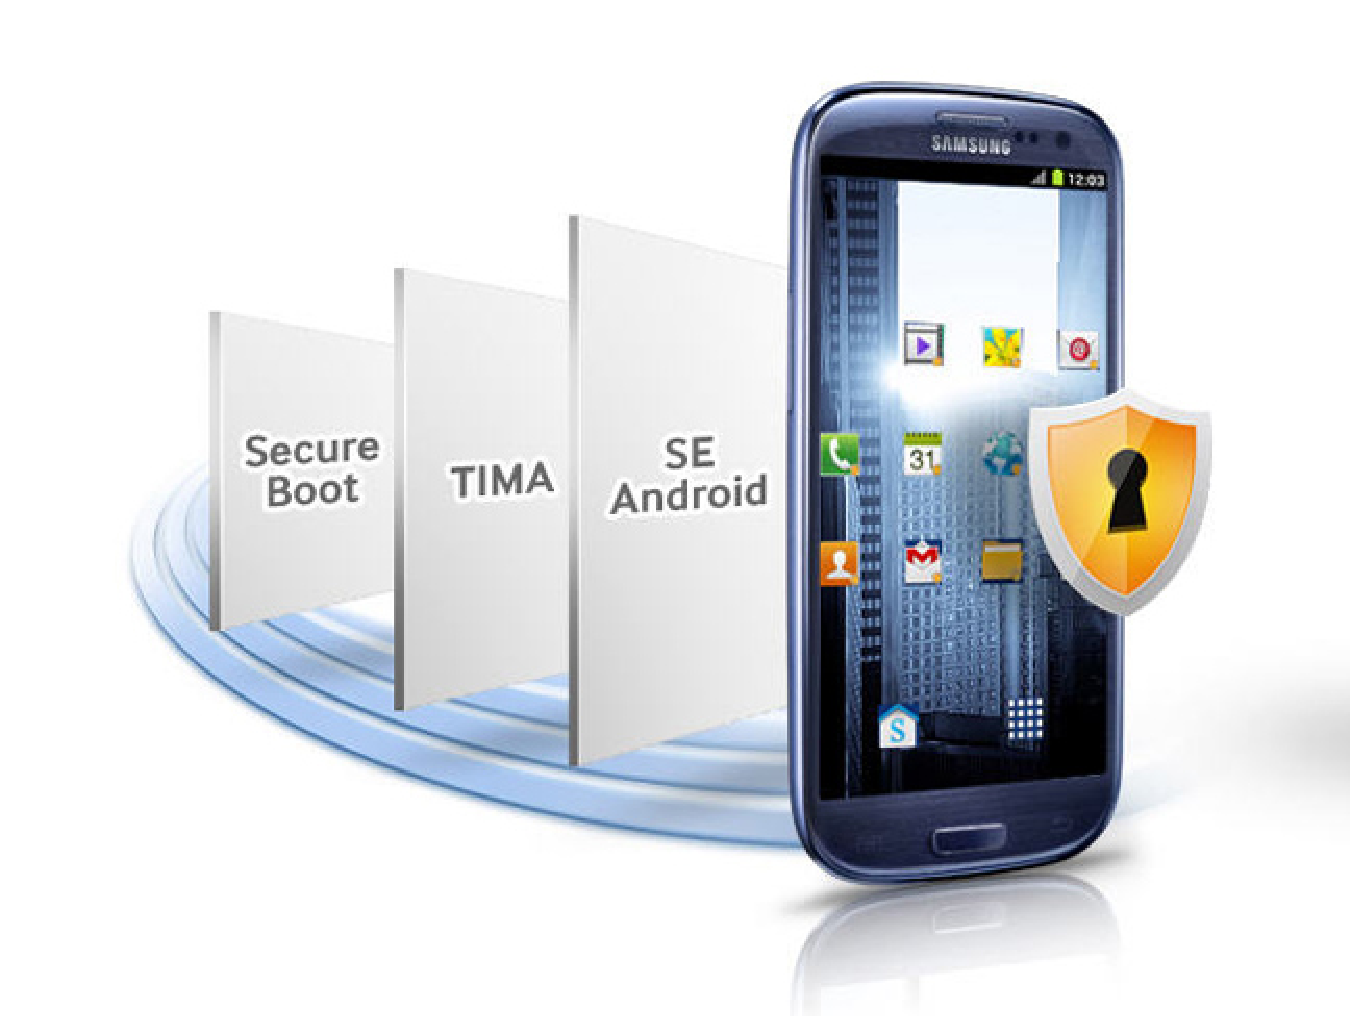
\includegraphics[scale=0.3]{img/samsung_knox_nueva.eps}
		\caption{Samsung's Knox utility architecture. Source: \url{http://www.samsung.com/global/business/mobile/solution/security/samsung-knox}.
	\label{fig:img_knox_01}
	\end{center}
\end{figure}

%----------------------------------------------------------------------------
\subsection{BlackBerry Balance}
\label{subsec:blackberrybalance}

This security package was announced as a feature of BlackBerry 10. Nevertheless, it is available with BlackBerry Enterprise Service 10, which is a device management, security and app management for BlackBerry, iOS and Android devices. When BlackBerry Balance it is activated, these characteristics are available:

\begin{enumerate}
	\item Work data cannot be copied and pasted into personal apps. The device will display messages like the shown in Figure \ref{fig:blackberry_bal}.
	\item If a user attempts an action that is not permitted by IT policy or that may cause secure work information to come into contact with personal applications, the action won't be permitted.
	\item Employees can access the personal information and apps that keep them in touch with the people and things they care about, while staying connected to important work information when they need to perform.
	\item If the device gets lost or stolen, or if the employee leaves the organization, there will be an option to wipe just work information and it can be done remotely.
\end{enumerate}


\begin{figure}
	\centering
		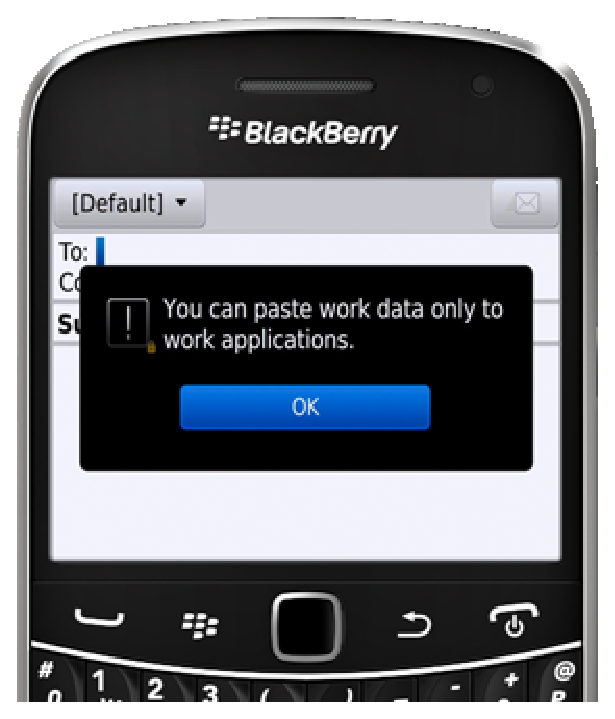
\includegraphics[scale=0.5]{img/Blackberry_balance.eps}
		\caption{Displayed message in new Blackberry 10 when attepmting to copy sensitive company data. Source: \url{http://uk.blackberry.com/business/software/blackberry-balance.html}.
	\label{fig:blackberry_bal}
\end{figure}

%----------------------------------------------------------------------------
\subsection{Multiplatform Usable Endpoint Security}
\label{subsec:muses}

MUSES (or Multiplatform Usable Endpoint Security) is a project co-funded by the European Commission under the Seventh Framework Programme. This MUSES project has concluded it first year (from a total of three) and is expected to develop a prototype (Prototype #1) for Android Devices in the second year.
The final product of MUSES for companies will be a system which will be installed in workers' devices and enterprise servers. There will be compiled versions of MUSES deployed on these kinds of devices:

\begin{enumerate}
	\item Portable devices. These are laptops that can be used in the company's premises or elsewhere.
	\item Mobile devices. These include smartphones and tablets.
	\item Enterprise servers.
\end{enumerate}
	
The first two kinds can be owned either by the company itself or their employees (or their co-workers, where co-workers are indirect employees of the company; the term generally refers to the employees of contractor companies.).
The very definition of MUSES as multiplatform usable endpoint security implies that the MUSES solution should be deployable and run on a number of platforms and operating systems. Being multiplatform is a key requirement for the adoption of MUSES as part of a wide range of corporate security strategies.

In order to achieve its stated goals the MUSES system should be able to: capture user's behaviour, decide in real-time if user's behaviour poses a security threat, propose adaptations of the security policies based on patterns of user's behaviour, provide usable feedback to the user (based on security threat), and apply necessary adaptations and manipulation of context.


%%%%%%%%%%%%%%%%%%%%%%%%%%%%%  CONCLUSIONS %%%%%%%%%%%%%%%%%%%%%%%%%%%%%%%%

\section{Conclusions}
\label{sec:conclusions}

In this work, there have been presented many tools that prove how information security in the enterprise is adapting to this emergent philosophy of BYOD. We have shown how the European Community is specially aware about that and is developing a free solution for managing employees privacy, and securing companies' assets in this changing environment. 

\section*{Acknowledgements}
This work has been supported by MUSES FP7 project, and in part by the P08-TIC-03903 project awarded by the Andalusian Regional Government, the FPU Grant 2009-2942 and the TIN2011-28627-C04-02 project, awarded by the Spanish Ministry of Science and Innovation.

\bibliographystyle{splncs}

\begin{thebibliography}{00}

\bibitem{EAs_Back96}
B\"ack, T., \emph{Evolutionary algorithms in theory and practice}, Oxford University Press, 1996.

\bibitem{SuperMario_Astar}
R. Baumgarten, \emph{Mario AI A* agent},
http://www.doc.ic.ac.uk/~rb1006/projects:marioai.

\bibitem{SuperMario_rulebased}
Bojarski, S., Bates-Congdon, C., \emph{REALM: A Rule-Based Evolutionary Computation Agent that Learns to Play Mario}. In: Proceedings of the 2011 IEEE Symposium on Computational Intelligence and Games (CIG 2011), IEEE Press, pp. 83--90, 2011. 

\bibitem{FSM_Booth}
Booth, T.L., \emph{Sequential Machines and Automata Theory}, John Wiley and Sons, Inc., New York, 1st edition, 1967.

%\bibitem{ControllingBot_CEC2010}
%Esparcia-Alc{\'a}zar A I, Mart�nez-Garc\'{\i}a A I, Mora A M, Merelo J J, Garc\'{\i}a-S{\'a}nchez P. Controlling bots in a first person shooter game using genetic algorithms. In \emph{Proc. 2010 IEEE Congress on Evolutionary Computation (CEC 2010)}, July 2010, pp. 1--8.

\bibitem{GAs_Goldberg89}
Goldberg D.E., Korb B., Deb K., \emph{Messy genetic algorithms: motivation, analysis, and first results}, Complex Systems, 3(5), pp. 493--530, 1989.

\bibitem{potfields_starcraft}
Hagelb\"ack, J., \emph{Potential-Field Based navigation in StarCraft}. In: Proceedings of the 2012 IEEE Symposium on Computational Intelligence and Games (CIG 2012), IEEE Press, pp. 388--393, 2012. 

\bibitem{optimalRTS}
Jang, S.H., Yoon, J.W., Cho, S.B., \emph{Optimal strategy selection of non-player character on real time strategy game using a speciated evolutionary algorithm}. In: Proceedings of the 5th IEEE Symposium on Computational Intelligence and Games (CIG'09), IEEE Press, pp. 75--79, 2009.

\bibitem{laird2001using}
Laird, J.E, \emph{Using a computer game to develop advanced AI}.
  Computer, 34(7), pp. 70--75, 2001.

\bibitem{Pac-MAnt_CIG2010}
Mart�n, E., Mart�nez, M., Recio, G., Saez, Y., \emph{{Pac-mAnt}: Optimization based on ant colonies applied to developing an agent for Ms. Pac-Man}. In Proc. 2010 IEEE Conference on Computational Intelligence and Games (CIG 2010), IEEE Press, pp. 458--464, 2010.

\bibitem{cooperativebots_CIG2010}
Mora, A.M., Moreno, M.A., Merelo, J.J., Castillo, P.A., Garc�a-Arenas, M.I., Laredo, J.L.J., \emph{Evolving the cooperative behaviour in {Unreal}\texttrademark~ bots}. In Proc. 2010 IEEE Conference on Computational Intelligence and Games (CIG 2010), IEEE Press, pp. 241--248, 2010.

\bibitem{noisyfitness_EVO2012}
Mora, A.M., Fern�ndez-Ares, A., Merelo, J.J., Garc�a-S�nchez, P., \emph{Dealing with noisy fitness in the design of a RTS game bot}. In Proc. Applications of Evolutionary Computing: EvoApplications 2012, LNCS, vol. 7248, Springer, pp. 234--244, 2012.

\bibitem{SuperMario_playerexperience}
Pedersen, C., Togelius, J., Yannakakis, G., \emph{Modeling Player Experience in Super Mario Bros}. In Proc. 2009 IEEE Symposium on Computational Intelligence and Games (CIG'09), IEEE Press, pp 132--139, 2009.

\bibitem{MTCS_PacMan}
Pepels, T., Windans, H.M., \emph{Enhancements for Monte-Carlo Tree Search in Ms Pac-Man}. In Proc. 2012 IEEE Conference on Computational Intelligence and Games (CIG 2012), IEEE Press, pp. 265--272, 2012.

\bibitem{tactics_evolutionary_learning}
Ponsen, M., Munoz-Avila, H., Spronck, P., Aha, D.W., \emph{Automatically generating game tactics through evolutionary learning}. AI Magazine, 27(3), pp. 75--84, 2006.

\bibitem{SuperMario_levelgeneration}
Shaker, N., Nicolau M., Yannakakis, G.N., Togelius, J., O\textquoteright neill, M., \emph{Evolving Levels for Super Mario Bros Using Grammatical Evolution}. In Proc. 2012 IEEE Symposium on Computational Intelligence and Games (CIG 2012), IEEE Press, pp 304--311, 2012.

\bibitem{Agent_Smith_CEC2009}
Small, R., Bates-Congdon, C. \emph{Agent {S}mith: Towards an evolutionary
  rule-based agent for interactive dynamic games}. In Proc. 2009 IEEE Congress on Evolutionary Computation (CEC'09), pp. 660--666, 2009.

\bibitem{evolutionary_learning-offline}
Spronck, P., Sprinkhuizen-Kuyper, I., Postma, E., \emph{Improving opponent intelligence through offline evolutionary learning}. International Journal of Intelligent Games and Simulation, 2(1), pp. 20--27, 2003.

\bibitem{starcraft_bayesianmodel}
Synnaeve, G., Bessi�re, P., \emph{A Bayesian Model for RTS Units Control applied to StarCraft}. In Proc. 2011 IEEE Symposium on Computational Intelligence and Games (CIG 2011), IEEE Press, pp 190--196, 2011.

\bibitem{SuperMario_Togelius}
Togelius, J., Karakovskiy, S., Koutnik, J., Schmidhuber, J., \emph{Super Mario
  evolution}. In Proc. 2009 IEEE Symposium on Computational Intelligence and Games (CIG'09), IEEE Press, pp 156--161, 2009.

\end{thebibliography}

\end{document}


% VIDEOS:
%
% dif 12 -> stacked: http://www.youtube.com/watch?v=zNGfBApX7sk
% dif 12 (20 seconds): http://www.youtube.com/watch?v=46yK4laTU0E
% dif 3 -> passed: http://www.youtube.com/watch?v=qQVQ43sWwYY
% dif 2 -> passed: http://www.youtube.com/watch?v=gtfuY-L0WDA
% dif 1 -> passed: http://www.youtube.com/watch?v=6Pj6dZCE070
